\documentclass[twoside]{book}

% Packages required by doxygen
\usepackage{fixltx2e}
\usepackage{calc}
\usepackage{doxygen}
\usepackage[export]{adjustbox} % also loads graphicx
\usepackage{graphicx}
\usepackage[utf8]{inputenc}
\usepackage{makeidx}
\usepackage{multicol}
\usepackage{multirow}
\PassOptionsToPackage{warn}{textcomp}
\usepackage{textcomp}
\usepackage[nointegrals]{wasysym}
\usepackage[table]{xcolor}

% NLS support packages
\usepackage[T2A]{fontenc}
\usepackage[magyar]{babel}

% Font selection
\usepackage[T1]{fontenc}
\usepackage[scaled=.90]{helvet}
\usepackage{courier}
\usepackage{amssymb}
\usepackage{sectsty}
\renewcommand{\familydefault}{\sfdefault}
\allsectionsfont{%
  \fontseries{bc}\selectfont%
  \color{darkgray}%
}
\renewcommand{\DoxyLabelFont}{%
  \fontseries{bc}\selectfont%
  \color{darkgray}%
}
\newcommand{\+}{\discretionary{\mbox{\scriptsize$\hookleftarrow$}}{}{}}

% Page & text layout
\usepackage{geometry}
\geometry{%
  a4paper,%
  top=2.5cm,%
  bottom=2.5cm,%
  left=2.5cm,%
  right=2.5cm%
}
\tolerance=750
\hfuzz=15pt
\hbadness=750
\setlength{\emergencystretch}{15pt}
\setlength{\parindent}{0cm}
\setlength{\parskip}{3ex plus 2ex minus 2ex}
\makeatletter
\renewcommand{\paragraph}{%
  \@startsection{paragraph}{4}{0ex}{-1.0ex}{1.0ex}{%
    \normalfont\normalsize\bfseries\SS@parafont%
  }%
}
\renewcommand{\subparagraph}{%
  \@startsection{subparagraph}{5}{0ex}{-1.0ex}{1.0ex}{%
    \normalfont\normalsize\bfseries\SS@subparafont%
  }%
}
\makeatother

% Headers & footers
\usepackage{fancyhdr}
\pagestyle{fancyplain}
\fancyhead[LE]{\fancyplain{}{\bfseries\thepage}}
\fancyhead[CE]{\fancyplain{}{}}
\fancyhead[RE]{\fancyplain{}{\bfseries\leftmark}}
\fancyhead[LO]{\fancyplain{}{\bfseries\rightmark}}
\fancyhead[CO]{\fancyplain{}{}}
\fancyhead[RO]{\fancyplain{}{\bfseries\thepage}}
\fancyfoot[LE]{\fancyplain{}{}}
\fancyfoot[CE]{\fancyplain{}{}}
\fancyfoot[RE]{\fancyplain{}{\bfseries\scriptsize Készítette Doxygen }}
\fancyfoot[LO]{\fancyplain{}{\bfseries\scriptsize Készítette Doxygen }}
\fancyfoot[CO]{\fancyplain{}{}}
\fancyfoot[RO]{\fancyplain{}{}}
\renewcommand{\footrulewidth}{0.4pt}
\renewcommand{\chaptermark}[1]{%
  \markboth{#1}{}%
}
\renewcommand{\sectionmark}[1]{%
  \markright{\thesection\ #1}%
}

% Indices & bibliography
\usepackage{natbib}
\usepackage[titles]{tocloft}
\setcounter{tocdepth}{3}
\setcounter{secnumdepth}{5}
\makeindex

% Hyperlinks (required, but should be loaded last)
\usepackage{ifpdf}
\ifpdf
  \usepackage[pdftex,pagebackref=true]{hyperref}
\else
  \usepackage[ps2pdf,pagebackref=true]{hyperref}
\fi
\hypersetup{%
  colorlinks=true,%
  linkcolor=blue,%
  citecolor=blue,%
  unicode%
}

% Custom commands
\newcommand{\clearemptydoublepage}{%
  \newpage{\pagestyle{empty}\cleardoublepage}%
}

\usepackage{caption}
\captionsetup{labelsep=space,justification=centering,font={bf},singlelinecheck=off,skip=4pt,position=top}

%===== C O N T E N T S =====

\begin{document}

% Titlepage & ToC
\hypersetup{pageanchor=false,
             bookmarksnumbered=true,
             pdfencoding=unicode
            }
\pagenumbering{roman}
\begin{titlepage}
\vspace*{7cm}
\begin{center}%
{\Large Italrecept }\\
\vspace*{1cm}
{\large Készítette Doxygen 1.8.11}\\
\end{center}
\end{titlepage}
\clearemptydoublepage
\tableofcontents
\clearemptydoublepage
\pagenumbering{arabic}
\hypersetup{pageanchor=true}

%--- Begin generated contents ---
\chapter{Adatszerkezet-\/mutató}
\section{Adatszerkezetek}
Az összes adatszerkezet listája rövid leírásokkal\+:\begin{DoxyCompactList}
\item\contentsline{section}{\hyperlink{classAlapanyag}{Alapanyag} }{\pageref{classAlapanyag}}{}
\item\contentsline{section}{\hyperlink{classHozzavalo}{Hozzavalo} }{\pageref{classHozzavalo}}{}
\item\contentsline{section}{\hyperlink{classLista}{Lista$<$ T\+I\+P\+U\+S $>$} }{\pageref{classLista}}{}
\item\contentsline{section}{\hyperlink{classRecept}{Recept} }{\pageref{classRecept}}{}
\end{DoxyCompactList}

\chapter{Fájlmutató}
\section{Fájllista}
Az összes fájl listája rövid leírásokkal\+:\begin{DoxyCompactList}
\item\contentsline{section}{\hyperlink{main_8cpp}{main.\+cpp} }{\pageref{main_8cpp}}{}
\item\contentsline{section}{\hyperlink{osztalyok_8hpp}{osztalyok.\+hpp} }{\pageref{osztalyok_8hpp}}{}
\end{DoxyCompactList}

\chapter{Adatszerkezetek dokumentációja}
\hypertarget{classAlapanyag}{}\section{Alapanyag osztályreferencia}
\label{classAlapanyag}\index{Alapanyag@{Alapanyag}}


{\ttfamily \#include $<$osztalyok.\+hpp$>$}



Az Alapanyag osztály együttműködési diagramja\+:\nopagebreak
\begin{figure}[H]
\begin{center}
\leavevmode
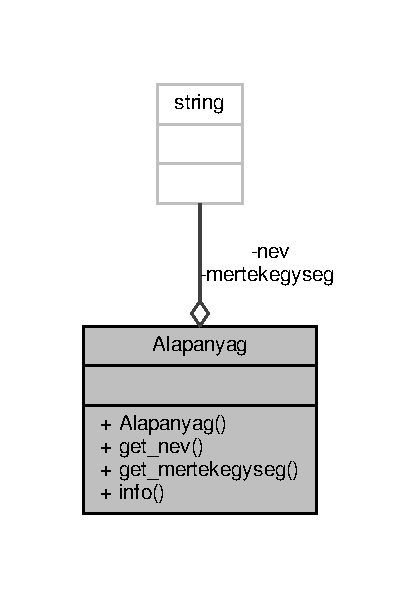
\includegraphics[width=201pt]{classAlapanyag__coll__graph}
\end{center}
\end{figure}
\subsection*{Publikus tagfüggvények}
\begin{DoxyCompactItemize}
\item 
\hyperlink{classAlapanyag_ac50b052225836ada3e16d4b1624d885b}{Alapanyag} (std\+::string \hyperlink{classAlapanyag_a9c1f11bb5b17c2c897b8f3b9a6a8e502}{nev}, std\+::string \hyperlink{classAlapanyag_aa0bf609f16b9bcd79ba888991f01e48b}{mertekegyseg})
\item 
std\+::string \hyperlink{classAlapanyag_a77fde4a6af30c5fd1a95817b6c6804bb}{get\+\_\+nev} () const 
\item 
std\+::string \hyperlink{classAlapanyag_ad55d9eb66d0c958d5c38c716776cb7be}{get\+\_\+mertekegyseg} () const 
\item 
void \hyperlink{classAlapanyag_afb76b8324db797a066224f841d95bd47}{info} (std\+::ostream os) const 
\end{DoxyCompactItemize}
\subsection*{Privát attribútumok}
\begin{DoxyCompactItemize}
\item 
std\+::string \hyperlink{classAlapanyag_a9c1f11bb5b17c2c897b8f3b9a6a8e502}{nev}
\item 
std\+::string \hyperlink{classAlapanyag_aa0bf609f16b9bcd79ba888991f01e48b}{mertekegyseg}
\end{DoxyCompactItemize}


\subsection{Részletes leírás}
A recepthez szükséges hozzávalók alapanyagokból építhetőek fel, de alapanyag önmagában is létezhet recept nélkül 

Definíció a(z) osztalyok.\+hpp fájl 9. sorában.



\subsection{Konstruktorok és destruktorok dokumentációja}
\index{Alapanyag@{Alapanyag}!Alapanyag@{Alapanyag}}
\index{Alapanyag@{Alapanyag}!Alapanyag@{Alapanyag}}
\subsubsection[{\texorpdfstring{Alapanyag(std\+::string nev, std\+::string mertekegyseg)}{Alapanyag(std::string nev, std::string mertekegyseg)}}]{\setlength{\rightskip}{0pt plus 5cm}Alapanyag\+::\+Alapanyag (
\begin{DoxyParamCaption}
\item[{std\+::string}]{nev, }
\item[{std\+::string}]{mertekegyseg}
\end{DoxyParamCaption}
)\hspace{0.3cm}{\ttfamily [inline]}}\hypertarget{classAlapanyag_ac50b052225836ada3e16d4b1624d885b}{}\label{classAlapanyag_ac50b052225836ada3e16d4b1624d885b}
\hyperlink{classAlapanyag}{Alapanyag} mértékegysége 

Definíció a(z) osztalyok.\+hpp fájl 14. sorában.



\subsection{Tagfüggvények dokumentációja}
\index{Alapanyag@{Alapanyag}!get\+\_\+mertekegyseg@{get\+\_\+mertekegyseg}}
\index{get\+\_\+mertekegyseg@{get\+\_\+mertekegyseg}!Alapanyag@{Alapanyag}}
\subsubsection[{\texorpdfstring{get\+\_\+mertekegyseg() const }{get_mertekegyseg() const }}]{\setlength{\rightskip}{0pt plus 5cm}std\+::string Alapanyag\+::get\+\_\+mertekegyseg (
\begin{DoxyParamCaption}
{}
\end{DoxyParamCaption}
) const\hspace{0.3cm}{\ttfamily [inline]}}\hypertarget{classAlapanyag_ad55d9eb66d0c958d5c38c716776cb7be}{}\label{classAlapanyag_ad55d9eb66d0c958d5c38c716776cb7be}


Definíció a(z) osztalyok.\+hpp fájl 16. sorában.

\index{Alapanyag@{Alapanyag}!get\+\_\+nev@{get\+\_\+nev}}
\index{get\+\_\+nev@{get\+\_\+nev}!Alapanyag@{Alapanyag}}
\subsubsection[{\texorpdfstring{get\+\_\+nev() const }{get_nev() const }}]{\setlength{\rightskip}{0pt plus 5cm}std\+::string Alapanyag\+::get\+\_\+nev (
\begin{DoxyParamCaption}
{}
\end{DoxyParamCaption}
) const\hspace{0.3cm}{\ttfamily [inline]}}\hypertarget{classAlapanyag_a77fde4a6af30c5fd1a95817b6c6804bb}{}\label{classAlapanyag_a77fde4a6af30c5fd1a95817b6c6804bb}


Definíció a(z) osztalyok.\+hpp fájl 15. sorában.

\index{Alapanyag@{Alapanyag}!info@{info}}
\index{info@{info}!Alapanyag@{Alapanyag}}
\subsubsection[{\texorpdfstring{info(std\+::ostream os) const }{info(std::ostream os) const }}]{\setlength{\rightskip}{0pt plus 5cm}void Alapanyag\+::info (
\begin{DoxyParamCaption}
\item[{std\+::ostream}]{os}
\end{DoxyParamCaption}
) const\hspace{0.3cm}{\ttfamily [inline]}}\hypertarget{classAlapanyag_afb76b8324db797a066224f841d95bd47}{}\label{classAlapanyag_afb76b8324db797a066224f841d95bd47}


Definíció a(z) osztalyok.\+hpp fájl 17. sorában.



\subsection{Adatmezők dokumentációja}
\index{Alapanyag@{Alapanyag}!mertekegyseg@{mertekegyseg}}
\index{mertekegyseg@{mertekegyseg}!Alapanyag@{Alapanyag}}
\subsubsection[{\texorpdfstring{mertekegyseg}{mertekegyseg}}]{\setlength{\rightskip}{0pt plus 5cm}std\+::string Alapanyag\+::mertekegyseg\hspace{0.3cm}{\ttfamily [private]}}\hypertarget{classAlapanyag_aa0bf609f16b9bcd79ba888991f01e48b}{}\label{classAlapanyag_aa0bf609f16b9bcd79ba888991f01e48b}
\hyperlink{classAlapanyag}{Alapanyag} neve 

Definíció a(z) osztalyok.\+hpp fájl 12. sorában.

\index{Alapanyag@{Alapanyag}!nev@{nev}}
\index{nev@{nev}!Alapanyag@{Alapanyag}}
\subsubsection[{\texorpdfstring{nev}{nev}}]{\setlength{\rightskip}{0pt plus 5cm}std\+::string Alapanyag\+::nev\hspace{0.3cm}{\ttfamily [private]}}\hypertarget{classAlapanyag_a9c1f11bb5b17c2c897b8f3b9a6a8e502}{}\label{classAlapanyag_a9c1f11bb5b17c2c897b8f3b9a6a8e502}


Definíció a(z) osztalyok.\+hpp fájl 11. sorában.



Ez a dokumentáció az osztályról a következő fájl alapján készült\+:\begin{DoxyCompactItemize}
\item 
\hyperlink{osztalyok_8hpp}{osztalyok.\+hpp}\end{DoxyCompactItemize}

\hypertarget{classHozzavalo}{}\section{Hozzavalo osztályreferencia}
\label{classHozzavalo}\index{Hozzavalo@{Hozzavalo}}


{\ttfamily \#include $<$osztalyok.\+hpp$>$}



A Hozzavalo osztály együttműködési diagramja\+:\nopagebreak
\begin{figure}[H]
\begin{center}
\leavevmode
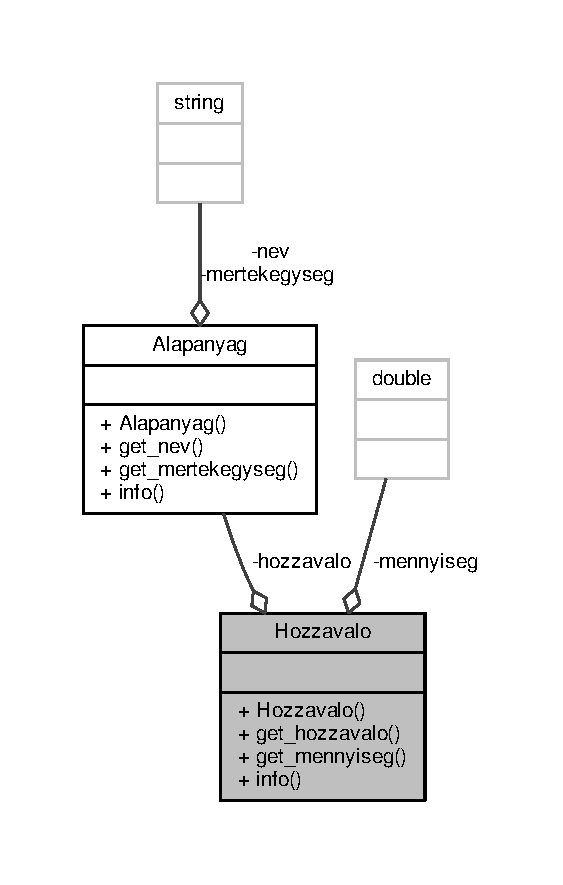
\includegraphics[width=270pt]{classHozzavalo__coll__graph}
\end{center}
\end{figure}
\subsection*{Publikus tagfüggvények}
\begin{DoxyCompactItemize}
\item 
\hyperlink{classHozzavalo_a616fae4cb079c68990413ecd8c8b97a6}{Hozzavalo} (\hyperlink{classAlapanyag}{Alapanyag} \hyperlink{classHozzavalo_ac2fd17dda552803cb220e9ea22be6793}{hozzavalo}, double \hyperlink{classHozzavalo_a31c9579b4bd274ef7ad5e934a90e0780}{mennyiseg})
\item 
\hyperlink{classAlapanyag}{Alapanyag} \hyperlink{classHozzavalo_adcb8f8c51e9ec20c3e106846b2143c3a}{get\+\_\+hozzavalo} () const 
\item 
double \hyperlink{classHozzavalo_a750b741dfbbdcf1d54476c1d124f736c}{get\+\_\+mennyiseg} () const 
\item 
void \hyperlink{classHozzavalo_aee49a4ae7c61f37d1bfee9d5115db4ff}{info} (std\+::ostream os) const 
\end{DoxyCompactItemize}
\subsection*{Privát attribútumok}
\begin{DoxyCompactItemize}
\item 
\hyperlink{classAlapanyag}{Alapanyag} \hyperlink{classHozzavalo_ac2fd17dda552803cb220e9ea22be6793}{hozzavalo}
\item 
double \hyperlink{classHozzavalo_a31c9579b4bd274ef7ad5e934a90e0780}{mennyiseg}
\end{DoxyCompactItemize}


\subsection{Részletes leírás}
Egy konkrét receptben egy hozzávaló áll egy alapanyagból és hogy mekkora mennyiségre van szükség belőle az adott recepthez. 

Definíció a(z) osztalyok.\+hpp fájl 23. sorában.



\subsection{Konstruktorok és destruktorok dokumentációja}
\index{Hozzavalo@{Hozzavalo}!Hozzavalo@{Hozzavalo}}
\index{Hozzavalo@{Hozzavalo}!Hozzavalo@{Hozzavalo}}
\subsubsection[{\texorpdfstring{Hozzavalo(\+Alapanyag hozzavalo, double mennyiseg)}{Hozzavalo(Alapanyag hozzavalo, double mennyiseg)}}]{\setlength{\rightskip}{0pt plus 5cm}Hozzavalo\+::\+Hozzavalo (
\begin{DoxyParamCaption}
\item[{{\bf Alapanyag}}]{hozzavalo, }
\item[{double}]{mennyiseg}
\end{DoxyParamCaption}
)\hspace{0.3cm}{\ttfamily [inline]}}\hypertarget{classHozzavalo_a616fae4cb079c68990413ecd8c8b97a6}{}\label{classHozzavalo_a616fae4cb079c68990413ecd8c8b97a6}


Definíció a(z) osztalyok.\+hpp fájl 28. sorában.



\subsection{Tagfüggvények dokumentációja}
\index{Hozzavalo@{Hozzavalo}!get\+\_\+hozzavalo@{get\+\_\+hozzavalo}}
\index{get\+\_\+hozzavalo@{get\+\_\+hozzavalo}!Hozzavalo@{Hozzavalo}}
\subsubsection[{\texorpdfstring{get\+\_\+hozzavalo() const }{get_hozzavalo() const }}]{\setlength{\rightskip}{0pt plus 5cm}{\bf Alapanyag} Hozzavalo\+::get\+\_\+hozzavalo (
\begin{DoxyParamCaption}
{}
\end{DoxyParamCaption}
) const\hspace{0.3cm}{\ttfamily [inline]}}\hypertarget{classHozzavalo_adcb8f8c51e9ec20c3e106846b2143c3a}{}\label{classHozzavalo_adcb8f8c51e9ec20c3e106846b2143c3a}


Definíció a(z) osztalyok.\+hpp fájl 29. sorában.

\index{Hozzavalo@{Hozzavalo}!get\+\_\+mennyiseg@{get\+\_\+mennyiseg}}
\index{get\+\_\+mennyiseg@{get\+\_\+mennyiseg}!Hozzavalo@{Hozzavalo}}
\subsubsection[{\texorpdfstring{get\+\_\+mennyiseg() const }{get_mennyiseg() const }}]{\setlength{\rightskip}{0pt plus 5cm}double Hozzavalo\+::get\+\_\+mennyiseg (
\begin{DoxyParamCaption}
{}
\end{DoxyParamCaption}
) const\hspace{0.3cm}{\ttfamily [inline]}}\hypertarget{classHozzavalo_a750b741dfbbdcf1d54476c1d124f736c}{}\label{classHozzavalo_a750b741dfbbdcf1d54476c1d124f736c}


Definíció a(z) osztalyok.\+hpp fájl 30. sorában.

\index{Hozzavalo@{Hozzavalo}!info@{info}}
\index{info@{info}!Hozzavalo@{Hozzavalo}}
\subsubsection[{\texorpdfstring{info(std\+::ostream os) const }{info(std::ostream os) const }}]{\setlength{\rightskip}{0pt plus 5cm}void Hozzavalo\+::info (
\begin{DoxyParamCaption}
\item[{std\+::ostream}]{os}
\end{DoxyParamCaption}
) const\hspace{0.3cm}{\ttfamily [inline]}}\hypertarget{classHozzavalo_aee49a4ae7c61f37d1bfee9d5115db4ff}{}\label{classHozzavalo_aee49a4ae7c61f37d1bfee9d5115db4ff}


Definíció a(z) osztalyok.\+hpp fájl 31. sorában.



A függvény hívási gráfja\+:
\nopagebreak
\begin{figure}[H]
\begin{center}
\leavevmode
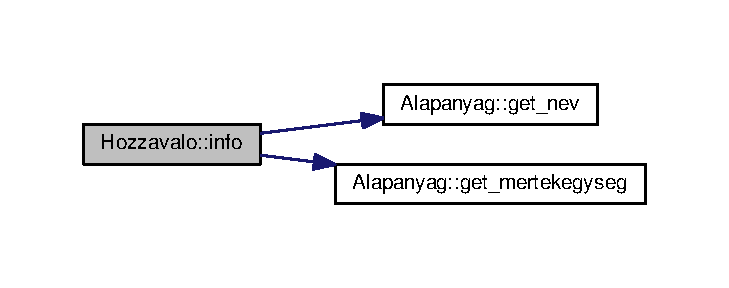
\includegraphics[width=350pt]{classHozzavalo_aee49a4ae7c61f37d1bfee9d5115db4ff_cgraph}
\end{center}
\end{figure}




\subsection{Adatmezők dokumentációja}
\index{Hozzavalo@{Hozzavalo}!hozzavalo@{hozzavalo}}
\index{hozzavalo@{hozzavalo}!Hozzavalo@{Hozzavalo}}
\subsubsection[{\texorpdfstring{hozzavalo}{hozzavalo}}]{\setlength{\rightskip}{0pt plus 5cm}{\bf Alapanyag} Hozzavalo\+::hozzavalo\hspace{0.3cm}{\ttfamily [private]}}\hypertarget{classHozzavalo_ac2fd17dda552803cb220e9ea22be6793}{}\label{classHozzavalo_ac2fd17dda552803cb220e9ea22be6793}


Definíció a(z) osztalyok.\+hpp fájl 25. sorában.

\index{Hozzavalo@{Hozzavalo}!mennyiseg@{mennyiseg}}
\index{mennyiseg@{mennyiseg}!Hozzavalo@{Hozzavalo}}
\subsubsection[{\texorpdfstring{mennyiseg}{mennyiseg}}]{\setlength{\rightskip}{0pt plus 5cm}double Hozzavalo\+::mennyiseg\hspace{0.3cm}{\ttfamily [private]}}\hypertarget{classHozzavalo_a31c9579b4bd274ef7ad5e934a90e0780}{}\label{classHozzavalo_a31c9579b4bd274ef7ad5e934a90e0780}


Definíció a(z) osztalyok.\+hpp fájl 26. sorában.



Ez a dokumentáció az osztályról a következő fájl alapján készült\+:\begin{DoxyCompactItemize}
\item 
\hyperlink{osztalyok_8hpp}{osztalyok.\+hpp}\end{DoxyCompactItemize}

\hypertarget{classLista}{}\section{Lista$<$ T\+I\+P\+US $>$ osztálysablon-\/referencia}
\label{classLista}\index{Lista$<$ T\+I\+P\+U\+S $>$@{Lista$<$ T\+I\+P\+U\+S $>$}}


{\ttfamily \#include $<$osztalyok.\+hpp$>$}



A Lista$<$ T\+I\+P\+US $>$ osztály együttműködési diagramja\+:\nopagebreak
\begin{figure}[H]
\begin{center}
\leavevmode
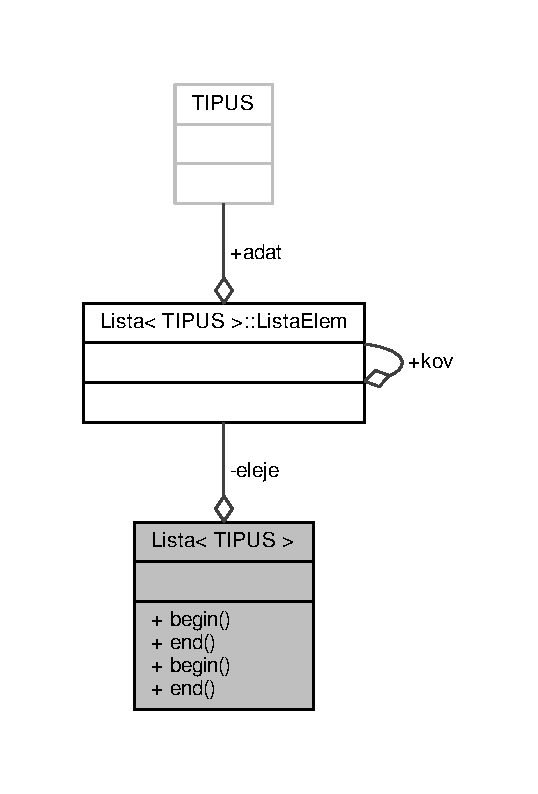
\includegraphics[width=258pt]{classLista__coll__graph}
\end{center}
\end{figure}
\subsection*{Adatszerkezetek}
\begin{DoxyCompactItemize}
\item 
class \hyperlink{classLista_classLista_1_1const__iterator}{const\+\_\+iterator}
\item 
class \hyperlink{classLista_classLista_1_1iterator}{iterator}
\item 
struct \hyperlink{classLista_structLista_1_1ListaElem}{Lista\+Elem}
\end{DoxyCompactItemize}
\subsection*{Publikus tagfüggvények}
\begin{DoxyCompactItemize}
\item 
\hyperlink{classLista_classLista_1_1iterator}{iterator} \hyperlink{classLista_ac32b6933b5c76f89b7f5f8f44690a3d0}{begin} ()
\item 
\hyperlink{classLista_classLista_1_1iterator}{iterator} \hyperlink{classLista_ae8ce80dee0b50fbb37fe097af7a333df}{end} ()
\item 
\hyperlink{classLista_classLista_1_1const__iterator}{const\+\_\+iterator} \hyperlink{classLista_a5de2207b484332b1c359bb753c894cc1}{begin} () const 
\item 
\hyperlink{classLista_classLista_1_1const__iterator}{const\+\_\+iterator} \hyperlink{classLista_ac277630e720e2f2a7519cc018b497773}{end} () const 
\end{DoxyCompactItemize}
\subsection*{Privát attribútumok}
\begin{DoxyCompactItemize}
\item 
\hyperlink{classLista_structLista_1_1ListaElem}{Lista\+Elem} $\ast$ \hyperlink{classLista_a3bf1edb5c453b6c959ccab89792e81f4}{eleje}
\end{DoxyCompactItemize}


\subsection{Részletes leírás}
\subsubsection*{template$<$typename T\+I\+P\+US$>$\\*
class Lista$<$ T\+I\+P\+U\+S $>$}

iterátoros láncolt lista. Két félére lesz szükség\+: Receptek és Alapanyagok tárolására. forrás\+: \href{http://cppftw.org/jegyzet/fejezet06.html#link5}{\tt http\+://cppftw.\+org/jegyzet/fejezet06.\+html\#link5} 

Definíció a(z) osztalyok.\+hpp fájl 55. sorában.



\subsection{Adatszerkezetek dokumentációja}
\index{Lista\+::const\+\_\+iterator@{Lista\+::const\+\_\+iterator}}\label{classLista_1_1const__iterator}
\hypertarget{classLista_classLista_1_1const__iterator}{}
\subsubsection{class Lista\+:\+:const\+\_\+iterator}
\subsubsection*{template$<$typename T\+I\+P\+US$>$\\*
class Lista$<$ T\+I\+P\+U\+S $>$\+::const\+\_\+iterator}



Definíció a(z) osztalyok.\+hpp fájl 66. sorában.



A Lista$<$ T\+I\+P\+US $>$\+:\+:const\+\_\+iterator osztály együttműködési diagramja\+:\nopagebreak
\begin{figure}[H]
\begin{center}
\leavevmode
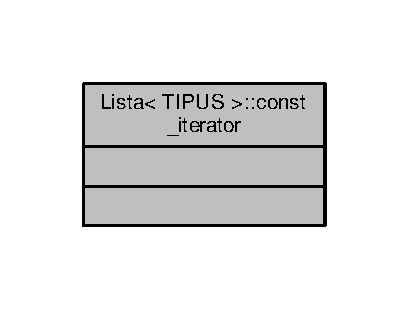
\includegraphics[width=196pt]{classLista_1_1const__iterator__coll__graph}
\end{center}
\end{figure}
\index{Lista\+::iterator@{Lista\+::iterator}}\label{classLista_1_1iterator}
\hypertarget{classLista_classLista_1_1iterator}{}
\subsubsection{class Lista\+:\+:iterator}
\subsubsection*{template$<$typename T\+I\+P\+US$>$\\*
class Lista$<$ T\+I\+P\+U\+S $>$\+::iterator}



Definíció a(z) osztalyok.\+hpp fájl 63. sorában.



A Lista$<$ T\+I\+P\+US $>$\+:\+:iterator osztály együttműködési diagramja\+:\nopagebreak
\begin{figure}[H]
\begin{center}
\leavevmode
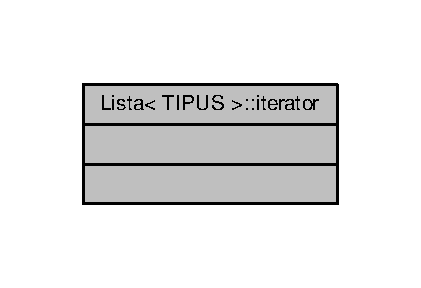
\includegraphics[width=202pt]{classLista_1_1iterator__coll__graph}
\end{center}
\end{figure}
\index{Lista\+::\+Lista\+Elem@{Lista\+::\+Lista\+Elem}}\label{structLista_1_1ListaElem}
\hypertarget{classLista_structLista_1_1ListaElem}{}
\subsubsection{struct Lista\+:\+:Lista\+Elem}
\subsubsection*{template$<$typename T\+I\+P\+US$>$\\*
struct Lista$<$ T\+I\+P\+U\+S $>$\+::\+Lista\+Elem}



Definíció a(z) osztalyok.\+hpp fájl 57. sorában.



A Lista$<$ T\+I\+P\+US $>$\+:\+:Lista\+Elem osztály együttműködési diagramja\+:\nopagebreak
\begin{figure}[H]
\begin{center}
\leavevmode
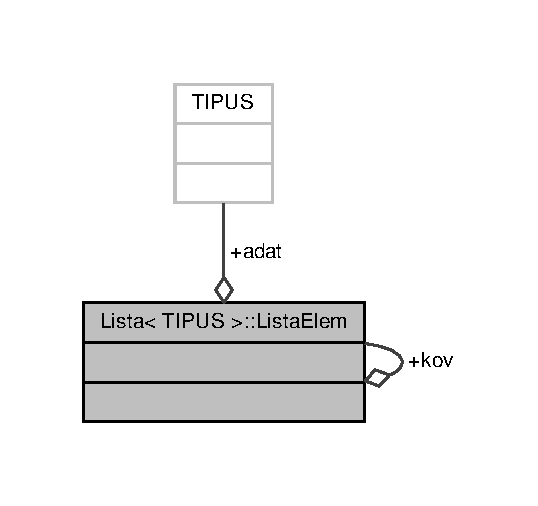
\includegraphics[width=258pt]{structLista_1_1ListaElem__coll__graph}
\end{center}
\end{figure}
\begin{DoxyFields}{Adatmezők}
T\+I\+P\+US\hypertarget{classLista_af3ebf30581a3eb36c4de08c2a08cd151}{}\label{classLista_af3ebf30581a3eb36c4de08c2a08cd151}
&
adat&
\\
\hline

\hyperlink{classLista_structLista_1_1ListaElem}{Lista\+Elem} $\ast$\hypertarget{classLista_a01e306c007ad116a02b89daae4003e92}{}\label{classLista_a01e306c007ad116a02b89daae4003e92}
&
kov&
\\
\hline

\end{DoxyFields}


\subsection{Tagfüggvények dokumentációja}
\index{Lista@{Lista}!begin@{begin}}
\index{begin@{begin}!Lista@{Lista}}
\subsubsection[{\texorpdfstring{begin()}{begin()}}]{\setlength{\rightskip}{0pt plus 5cm}template$<$typename T\+I\+P\+US $>$ {\bf iterator} {\bf Lista}$<$ T\+I\+P\+US $>$\+::begin (
\begin{DoxyParamCaption}
{}
\end{DoxyParamCaption}
)}\hypertarget{classLista_ac32b6933b5c76f89b7f5f8f44690a3d0}{}\label{classLista_ac32b6933b5c76f89b7f5f8f44690a3d0}
\index{Lista@{Lista}!begin@{begin}}
\index{begin@{begin}!Lista@{Lista}}
\subsubsection[{\texorpdfstring{begin() const }{begin() const }}]{\setlength{\rightskip}{0pt plus 5cm}template$<$typename T\+I\+P\+US $>$ {\bf const\+\_\+iterator} {\bf Lista}$<$ T\+I\+P\+US $>$\+::begin (
\begin{DoxyParamCaption}
{}
\end{DoxyParamCaption}
) const}\hypertarget{classLista_a5de2207b484332b1c359bb753c894cc1}{}\label{classLista_a5de2207b484332b1c359bb753c894cc1}
\index{Lista@{Lista}!end@{end}}
\index{end@{end}!Lista@{Lista}}
\subsubsection[{\texorpdfstring{end()}{end()}}]{\setlength{\rightskip}{0pt plus 5cm}template$<$typename T\+I\+P\+US $>$ {\bf iterator} {\bf Lista}$<$ T\+I\+P\+US $>$\+::end (
\begin{DoxyParamCaption}
{}
\end{DoxyParamCaption}
)}\hypertarget{classLista_ae8ce80dee0b50fbb37fe097af7a333df}{}\label{classLista_ae8ce80dee0b50fbb37fe097af7a333df}
\index{Lista@{Lista}!end@{end}}
\index{end@{end}!Lista@{Lista}}
\subsubsection[{\texorpdfstring{end() const }{end() const }}]{\setlength{\rightskip}{0pt plus 5cm}template$<$typename T\+I\+P\+US $>$ {\bf const\+\_\+iterator} {\bf Lista}$<$ T\+I\+P\+US $>$\+::end (
\begin{DoxyParamCaption}
{}
\end{DoxyParamCaption}
) const}\hypertarget{classLista_ac277630e720e2f2a7519cc018b497773}{}\label{classLista_ac277630e720e2f2a7519cc018b497773}


\subsection{Adatmezők dokumentációja}
\index{Lista@{Lista}!eleje@{eleje}}
\index{eleje@{eleje}!Lista@{Lista}}
\subsubsection[{\texorpdfstring{eleje}{eleje}}]{\setlength{\rightskip}{0pt plus 5cm}template$<$typename T\+I\+P\+US $>$ {\bf Lista\+Elem}$\ast$ {\bf Lista}$<$ T\+I\+P\+US $>$\+::eleje\hspace{0.3cm}{\ttfamily [private]}}\hypertarget{classLista_a3bf1edb5c453b6c959ccab89792e81f4}{}\label{classLista_a3bf1edb5c453b6c959ccab89792e81f4}


Definíció a(z) osztalyok.\+hpp fájl 61. sorában.



Ez a dokumentáció az osztályról a következő fájl alapján készült\+:\begin{DoxyCompactItemize}
\item 
\hyperlink{osztalyok_8hpp}{osztalyok.\+hpp}\end{DoxyCompactItemize}

\hypertarget{classRecept}{}\section{Recept osztályreferencia}
\label{classRecept}\index{Recept@{Recept}}


{\ttfamily \#include $<$osztalyok.\+hpp$>$}



A Recept osztály együttműködési diagramja\+:\nopagebreak
\begin{figure}[H]
\begin{center}
\leavevmode
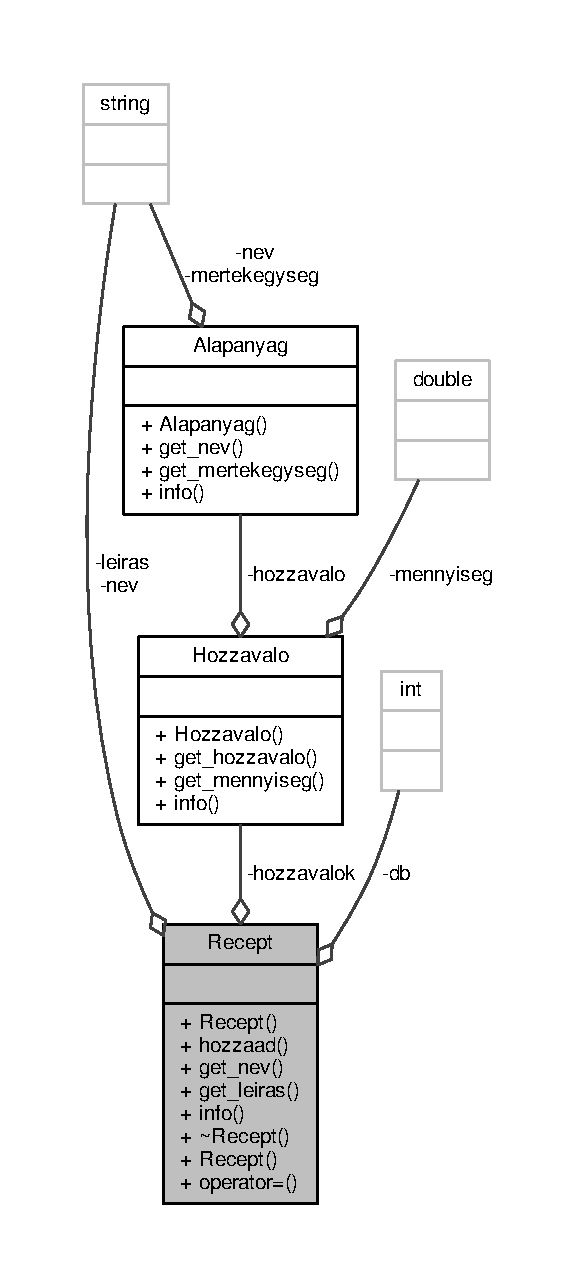
\includegraphics[height=550pt]{classRecept__coll__graph}
\end{center}
\end{figure}
\subsection*{Publikus tagfüggvények}
\begin{DoxyCompactItemize}
\item 
\hyperlink{classRecept_a9cdc66661e60cfe82d1c85e3640b505f}{Recept} (std\+::string \hyperlink{classRecept_afdc9105fc79f5027da1aebb6fd908b78}{nev}, std\+::string \hyperlink{classRecept_ab45575aab9abd31171cd35eb74665389}{leiras})
\item 
void \hyperlink{classRecept_a24ab7eb66a011f79e99bb2325148382e}{hozzaad} (\hyperlink{classHozzavalo}{Hozzavalo} const \&uj)
\item 
std\+::string \hyperlink{classRecept_a9936225342590bd721f477432fb162f4}{get\+\_\+nev} () const 
\item 
std\+::string \hyperlink{classRecept_a22e27d4afe257de56df8a84a5377f2af}{get\+\_\+leiras} () const 
\item 
void \hyperlink{classRecept_a2eccb11470a34650f8faad733960f66e}{info} (std\+::ostream os)
\item 
\hyperlink{classRecept_a53d1a6a6ae6983cd6e409051156535a4}{$\sim$\+Recept} ()
\item 
\hyperlink{classRecept_af73dd83922a0f5d9016d450bf1bd5d2c}{Recept} (\hyperlink{classRecept}{Recept} const \&r)
\item 
\hyperlink{classRecept}{Recept} \& \hyperlink{classRecept_adb6db4fde2bc6700b63a8750012be6b8}{operator=} (\hyperlink{classRecept}{Recept} const \&rhs)
\end{DoxyCompactItemize}
\subsection*{Privát attribútumok}
\begin{DoxyCompactItemize}
\item 
std\+::string \hyperlink{classRecept_afdc9105fc79f5027da1aebb6fd908b78}{nev}
\item 
std\+::string \hyperlink{classRecept_ab45575aab9abd31171cd35eb74665389}{leiras}
\item 
\hyperlink{classHozzavalo}{Hozzavalo} $\ast$ \hyperlink{classRecept_afb5204c5461622e25fd7c89da9874c01}{hozzavalok}
\item 
int \hyperlink{classRecept_a23e1d3a87bfdbd571a7641bd0b933eb8}{db}
\end{DoxyCompactItemize}


\subsection{Részletes leírás}
A név és leíráson kívül egy dinamikus tömbben tárolja a recept összetevőit 

Definíció a(z) osztalyok.\+hpp fájl 35. sorában.



\subsection{Konstruktorok és destruktorok dokumentációja}
\index{Recept@{Recept}!Recept@{Recept}}
\index{Recept@{Recept}!Recept@{Recept}}
\subsubsection[{\texorpdfstring{Recept(std\+::string nev, std\+::string leiras)}{Recept(std::string nev, std::string leiras)}}]{\setlength{\rightskip}{0pt plus 5cm}Recept\+::\+Recept (
\begin{DoxyParamCaption}
\item[{std\+::string}]{nev, }
\item[{std\+::string}]{leiras}
\end{DoxyParamCaption}
)\hspace{0.3cm}{\ttfamily [inline]}}\hypertarget{classRecept_a9cdc66661e60cfe82d1c85e3640b505f}{}\label{classRecept_a9cdc66661e60cfe82d1c85e3640b505f}
Mekkora a tömbök mérete 

Definíció a(z) osztalyok.\+hpp fájl 42. sorában.

\index{Recept@{Recept}!````~Recept@{$\sim$\+Recept}}
\index{````~Recept@{$\sim$\+Recept}!Recept@{Recept}}
\subsubsection[{\texorpdfstring{$\sim$\+Recept()}{~Recept()}}]{\setlength{\rightskip}{0pt plus 5cm}Recept\+::$\sim$\+Recept (
\begin{DoxyParamCaption}
{}
\end{DoxyParamCaption}
)\hspace{0.3cm}{\ttfamily [inline]}}\hypertarget{classRecept_a53d1a6a6ae6983cd6e409051156535a4}{}\label{classRecept_a53d1a6a6ae6983cd6e409051156535a4}


Definíció a(z) osztalyok.\+hpp fájl 47. sorában.

\index{Recept@{Recept}!Recept@{Recept}}
\index{Recept@{Recept}!Recept@{Recept}}
\subsubsection[{\texorpdfstring{Recept(\+Recept const \&r)}{Recept(Recept const &r)}}]{\setlength{\rightskip}{0pt plus 5cm}Recept\+::\+Recept (
\begin{DoxyParamCaption}
\item[{{\bf Recept} const \&}]{r}
\end{DoxyParamCaption}
)}\hypertarget{classRecept_af73dd83922a0f5d9016d450bf1bd5d2c}{}\label{classRecept_af73dd83922a0f5d9016d450bf1bd5d2c}


\subsection{Tagfüggvények dokumentációja}
\index{Recept@{Recept}!get\+\_\+leiras@{get\+\_\+leiras}}
\index{get\+\_\+leiras@{get\+\_\+leiras}!Recept@{Recept}}
\subsubsection[{\texorpdfstring{get\+\_\+leiras() const }{get_leiras() const }}]{\setlength{\rightskip}{0pt plus 5cm}std\+::string Recept\+::get\+\_\+leiras (
\begin{DoxyParamCaption}
{}
\end{DoxyParamCaption}
) const\hspace{0.3cm}{\ttfamily [inline]}}\hypertarget{classRecept_a22e27d4afe257de56df8a84a5377f2af}{}\label{classRecept_a22e27d4afe257de56df8a84a5377f2af}


Definíció a(z) osztalyok.\+hpp fájl 45. sorában.



A függvény hívási gráfja\+:
\nopagebreak
\begin{figure}[H]
\begin{center}
\leavevmode
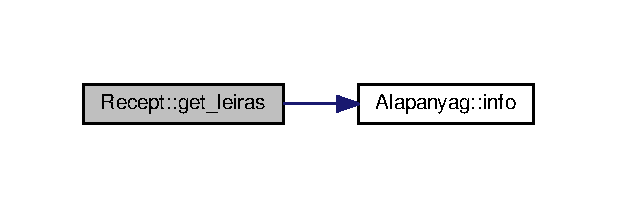
\includegraphics[width=296pt]{classRecept_a22e27d4afe257de56df8a84a5377f2af_cgraph}
\end{center}
\end{figure}


\index{Recept@{Recept}!get\+\_\+nev@{get\+\_\+nev}}
\index{get\+\_\+nev@{get\+\_\+nev}!Recept@{Recept}}
\subsubsection[{\texorpdfstring{get\+\_\+nev() const }{get_nev() const }}]{\setlength{\rightskip}{0pt plus 5cm}std\+::string Recept\+::get\+\_\+nev (
\begin{DoxyParamCaption}
{}
\end{DoxyParamCaption}
) const\hspace{0.3cm}{\ttfamily [inline]}}\hypertarget{classRecept_a9936225342590bd721f477432fb162f4}{}\label{classRecept_a9936225342590bd721f477432fb162f4}


Definíció a(z) osztalyok.\+hpp fájl 44. sorában.

\index{Recept@{Recept}!hozzaad@{hozzaad}}
\index{hozzaad@{hozzaad}!Recept@{Recept}}
\subsubsection[{\texorpdfstring{hozzaad(\+Hozzavalo const \&uj)}{hozzaad(Hozzavalo const &uj)}}]{\setlength{\rightskip}{0pt plus 5cm}void Recept\+::hozzaad (
\begin{DoxyParamCaption}
\item[{{\bf Hozzavalo} const \&}]{uj}
\end{DoxyParamCaption}
)}\hypertarget{classRecept_a24ab7eb66a011f79e99bb2325148382e}{}\label{classRecept_a24ab7eb66a011f79e99bb2325148382e}
\index{Recept@{Recept}!info@{info}}
\index{info@{info}!Recept@{Recept}}
\subsubsection[{\texorpdfstring{info(std\+::ostream os)}{info(std::ostream os)}}]{\setlength{\rightskip}{0pt plus 5cm}void Recept\+::info (
\begin{DoxyParamCaption}
\item[{std\+::ostream}]{os}
\end{DoxyParamCaption}
)}\hypertarget{classRecept_a2eccb11470a34650f8faad733960f66e}{}\label{classRecept_a2eccb11470a34650f8faad733960f66e}
\index{Recept@{Recept}!operator=@{operator=}}
\index{operator=@{operator=}!Recept@{Recept}}
\subsubsection[{\texorpdfstring{operator=(\+Recept const \&rhs)}{operator=(Recept const &rhs)}}]{\setlength{\rightskip}{0pt plus 5cm}{\bf Recept}\& Recept\+::operator= (
\begin{DoxyParamCaption}
\item[{{\bf Recept} const \&}]{rhs}
\end{DoxyParamCaption}
)}\hypertarget{classRecept_adb6db4fde2bc6700b63a8750012be6b8}{}\label{classRecept_adb6db4fde2bc6700b63a8750012be6b8}


\subsection{Adatmezők dokumentációja}
\index{Recept@{Recept}!db@{db}}
\index{db@{db}!Recept@{Recept}}
\subsubsection[{\texorpdfstring{db}{db}}]{\setlength{\rightskip}{0pt plus 5cm}int Recept\+::db\hspace{0.3cm}{\ttfamily [private]}}\hypertarget{classRecept_a23e1d3a87bfdbd571a7641bd0b933eb8}{}\label{classRecept_a23e1d3a87bfdbd571a7641bd0b933eb8}
Hozzavalok tömbje 

Definíció a(z) osztalyok.\+hpp fájl 40. sorában.

\index{Recept@{Recept}!hozzavalok@{hozzavalok}}
\index{hozzavalok@{hozzavalok}!Recept@{Recept}}
\subsubsection[{\texorpdfstring{hozzavalok}{hozzavalok}}]{\setlength{\rightskip}{0pt plus 5cm}{\bf Hozzavalo}$\ast$ Recept\+::hozzavalok\hspace{0.3cm}{\ttfamily [private]}}\hypertarget{classRecept_afb5204c5461622e25fd7c89da9874c01}{}\label{classRecept_afb5204c5461622e25fd7c89da9874c01}


Definíció a(z) osztalyok.\+hpp fájl 39. sorában.

\index{Recept@{Recept}!leiras@{leiras}}
\index{leiras@{leiras}!Recept@{Recept}}
\subsubsection[{\texorpdfstring{leiras}{leiras}}]{\setlength{\rightskip}{0pt plus 5cm}std\+::string Recept\+::leiras\hspace{0.3cm}{\ttfamily [private]}}\hypertarget{classRecept_ab45575aab9abd31171cd35eb74665389}{}\label{classRecept_ab45575aab9abd31171cd35eb74665389}


Definíció a(z) osztalyok.\+hpp fájl 38. sorában.

\index{Recept@{Recept}!nev@{nev}}
\index{nev@{nev}!Recept@{Recept}}
\subsubsection[{\texorpdfstring{nev}{nev}}]{\setlength{\rightskip}{0pt plus 5cm}std\+::string Recept\+::nev\hspace{0.3cm}{\ttfamily [private]}}\hypertarget{classRecept_afdc9105fc79f5027da1aebb6fd908b78}{}\label{classRecept_afdc9105fc79f5027da1aebb6fd908b78}


Definíció a(z) osztalyok.\+hpp fájl 37. sorában.



Ez a dokumentáció az osztályról a következő fájl alapján készült\+:\begin{DoxyCompactItemize}
\item 
\hyperlink{osztalyok_8hpp}{osztalyok.\+hpp}\end{DoxyCompactItemize}

\chapter{Fájlok dokumentációja}
\hypertarget{main_8cpp}{}\section{main.\+cpp fájlreferencia}
\label{main_8cpp}\index{main.\+cpp@{main.\+cpp}}
{\ttfamily \#include $<$iostream$>$}\\*
{\ttfamily \#include \char`\"{}osztalyok.\+hpp\char`\"{}}\\*
A main.\+cpp definíciós fájl függési gráfja\+:\nopagebreak
\begin{figure}[H]
\begin{center}
\leavevmode
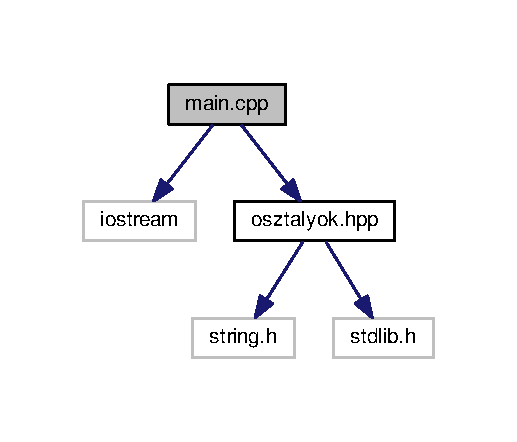
\includegraphics[width=248pt]{main_8cpp__incl}
\end{center}
\end{figure}
\subsection*{Függvények}
\begin{DoxyCompactItemize}
\item 
int \hyperlink{main_8cpp_ae66f6b31b5ad750f1fe042a706a4e3d4}{main} ()
\end{DoxyCompactItemize}


\subsection{Függvények dokumentációja}
\index{main.\+cpp@{main.\+cpp}!main@{main}}
\index{main@{main}!main.\+cpp@{main.\+cpp}}
\subsubsection[{\texorpdfstring{main()}{main()}}]{\setlength{\rightskip}{0pt plus 5cm}int main (
\begin{DoxyParamCaption}
{}
\end{DoxyParamCaption}
)}\hypertarget{main_8cpp_ae66f6b31b5ad750f1fe042a706a4e3d4}{}\label{main_8cpp_ae66f6b31b5ad750f1fe042a706a4e3d4}


Definíció a(z) main.\+cpp fájl 6. sorában.


\hypertarget{osztalyok_8hpp}{}\section{osztalyok.\+hpp fájlreferencia}
\label{osztalyok_8hpp}\index{osztalyok.\+hpp@{osztalyok.\+hpp}}
{\ttfamily \#include $<$string.\+h$>$}\\*
{\ttfamily \#include $<$stdlib.\+h$>$}\\*
Az osztalyok.\+hpp definíciós fájl függési gráfja\+:\nopagebreak
\begin{figure}[H]
\begin{center}
\leavevmode
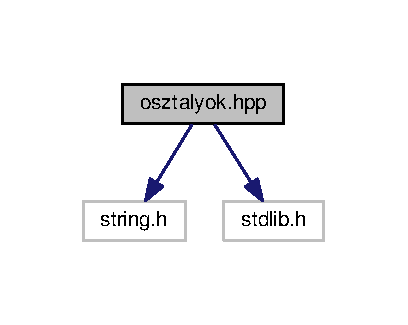
\includegraphics[width=196pt]{osztalyok_8hpp__incl}
\end{center}
\end{figure}
Ez az ábra azt mutatja, hogy mely fájlok ágyazzák be közvetve vagy közvetlenül ezt a fájlt\+:\nopagebreak
\begin{figure}[H]
\begin{center}
\leavevmode
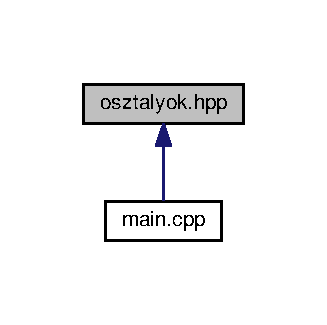
\includegraphics[width=157pt]{osztalyok_8hpp__dep__incl}
\end{center}
\end{figure}
\subsection*{Adatszerkezetek}
\begin{DoxyCompactItemize}
\item 
class \hyperlink{classAlapanyag}{Alapanyag}
\item 
class \hyperlink{classHozzavalo}{Hozzavalo}
\item 
class \hyperlink{classRecept}{Recept}
\item 
class \hyperlink{classLista}{Lista$<$ T\+I\+P\+U\+S $>$}
\item 
struct \hyperlink{classLista_structLista_1_1ListaElem}{Lista$<$ T\+I\+P\+U\+S $>$\+::\+Lista\+Elem}
\item 
class \hyperlink{classLista_classLista_1_1iterator}{Lista$<$ T\+I\+P\+U\+S $>$\+::iterator}
\item 
class \hyperlink{classLista_classLista_1_1const__iterator}{Lista$<$ T\+I\+P\+U\+S $>$\+::const\+\_\+iterator}
\end{DoxyCompactItemize}


\subsection{Adatszerkezetek dokumentációja}
\index{Lista\+::\+Lista\+Elem@{Lista\+::\+Lista\+Elem}}\label{structLista_1_1ListaElem}
\hypertarget{classLista_structLista_1_1ListaElem}{}
\subsubsection{struct Lista\+:\+:Lista\+Elem}
\subsubsection*{template$<$typename T\+I\+P\+US$>$\\*
struct Lista$<$ T\+I\+P\+U\+S $>$\+::\+Lista\+Elem}



Definíció a(z) osztalyok.\+hpp fájl 57. sorában.



A Lista$<$ T\+I\+P\+US $>$\+:\+:Lista\+Elem osztály együttműködési diagramja\+:\nopagebreak
\begin{figure}[H]
\begin{center}
\leavevmode
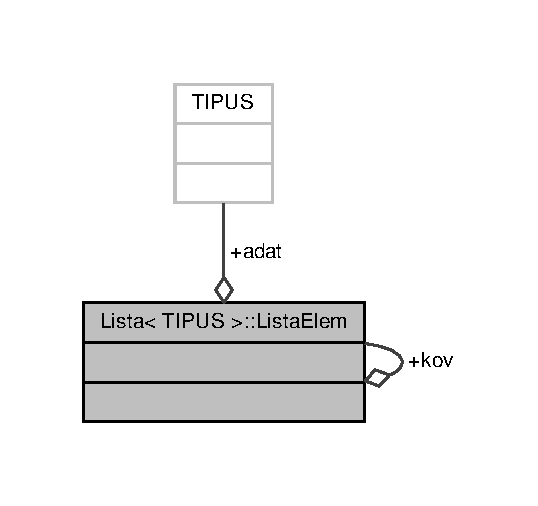
\includegraphics[width=258pt]{structLista_1_1ListaElem__coll__graph}
\end{center}
\end{figure}
\begin{DoxyFields}{Adatmezők}
T\+I\+P\+US\hypertarget{classLista_af3ebf30581a3eb36c4de08c2a08cd151}{}\label{classLista_af3ebf30581a3eb36c4de08c2a08cd151}
&
adat&
\\
\hline

\hyperlink{classLista_structLista_1_1ListaElem}{Lista\+Elem} $\ast$\hypertarget{classLista_a01e306c007ad116a02b89daae4003e92}{}\label{classLista_a01e306c007ad116a02b89daae4003e92}
&
kov&
\\
\hline

\end{DoxyFields}
\index{Lista\+::iterator@{Lista\+::iterator}}\label{classLista_1_1iterator}
\hypertarget{classLista_classLista_1_1iterator}{}
\subsubsection{class Lista\+:\+:iterator}
\subsubsection*{template$<$typename T\+I\+P\+US$>$\\*
class Lista$<$ T\+I\+P\+U\+S $>$\+::iterator}



Definíció a(z) osztalyok.\+hpp fájl 63. sorában.



A Lista$<$ T\+I\+P\+US $>$\+:\+:iterator osztály együttműködési diagramja\+:\nopagebreak
\begin{figure}[H]
\begin{center}
\leavevmode
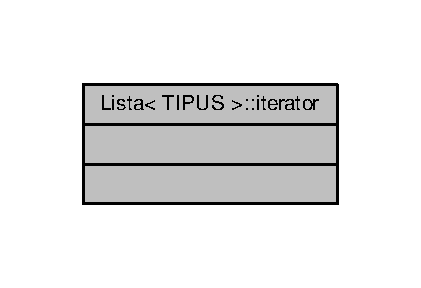
\includegraphics[width=202pt]{classLista_1_1iterator__coll__graph}
\end{center}
\end{figure}
\index{Lista\+::const\+\_\+iterator@{Lista\+::const\+\_\+iterator}}\label{classLista_1_1const__iterator}
\hypertarget{classLista_classLista_1_1const__iterator}{}
\subsubsection{class Lista\+:\+:const\+\_\+iterator}
\subsubsection*{template$<$typename T\+I\+P\+US$>$\\*
class Lista$<$ T\+I\+P\+U\+S $>$\+::const\+\_\+iterator}



Definíció a(z) osztalyok.\+hpp fájl 66. sorában.



A Lista$<$ T\+I\+P\+US $>$\+:\+:const\+\_\+iterator osztály együttműködési diagramja\+:\nopagebreak
\begin{figure}[H]
\begin{center}
\leavevmode
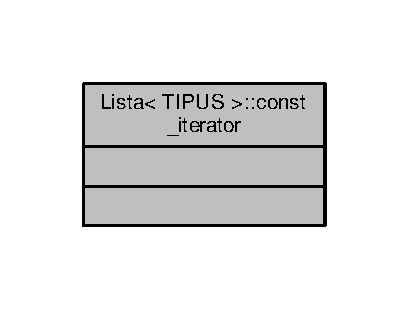
\includegraphics[width=196pt]{classLista_1_1const__iterator__coll__graph}
\end{center}
\end{figure}

%--- End generated contents ---

% Index
\backmatter
\newpage
\phantomsection
\clearemptydoublepage
\addcontentsline{toc}{chapter}{Tárgymutató}
\printindex

\end{document}
